
\citeasnoun{bushnell93motor} put forth the
claim that you can explain changes in infants' perceptual skills by
looking at what they're motorically capable of.  They discuss the
\cite{lederman87hand} Exploration Procedures and a few other examples in
some detail.  Their point about \citeasnoun{lederman87hand} was that until
babies/children are capable of producing the hand and arm movements
necessary for producing e.g., the up-and-down movements associated
with ``hefting'' thought to allow for the perception of object weight,
they're not going to perceive weight differences between objects.


\subsection{Robot stuff}

A strongly segmentable signal can be used to find more subtle signals.
Mapping from free-from signal to hypothesized segments is explosive
without strong filters, can mis a signal which, if suggested, would
be confirmable.  

A particularly segmentable signal is proprioception and efference copy. 


\subsection{Infant lead: role of behavior in the development of object segregations skills}

Evidence from of one set of studies reveals that young
infants' difficulty in collecting the relevant information
from visual displays may limit their success in these tasks (Johnson \&
Aslin 1995, \cite{johnson96perception}, then Johnson's eye tracking stuff
\cite{johnson04where} showing
that infants who look to the other side of the occluder, sampling
information from both sides of it, are the ones who perceive the
object parts as connected.  So, eye movements are an important factor
in this picture)

The changes in perception described throughout this section
do not occur in a vaccuum but rather in a
child who is also experiencing a range of other develomental changes.
One of these changes occurs in object
exploration -- infants' visual, oral, and manual
investigation of objects are showing huge improvements during this
same time period \cite{rochat89object}.  Relations between infants'
tendency to explore objects more or less actively and their accurate
parsing of an object display has been shown \cite{needham00improvements}, paving
the way for future studies of connections between object exploration
and object perception.


\section{Intermodal}







\subsection{Speech}

A special case of visual-auditory intermodal perception is speech
perception.  
%
In robotics and in speech recognition / computer vision, there's
a lot of interest in matching lip movement with speech sounds --
both to identify which of a set of people is speaking, and to
improve recognition performance by adding extra features.
%
We know that in adult humans, auditory and visual
information combine to create the speech sounds we hear (as evidenced
in the McGurk effect \cite{mcgurk76hearing}.  Evidence for the
McGurk effect has also been found in infants as young as 5 months of
age \cite{rosenblum97mcgurk}.  Young infants are able
to match the visual and auditory components of one particular speech
sound (e.g., they match an open mouthshape to the ``Ah'' sound and a
wide flat mouthshape to the ``Ee'' sound \cite{kuhl82bimodal}.
Detection of these multimodal correspondences facilitate infants'
identification of the appropriate speaker visually once the auditory
information is attended.

Movement of an object while a certain vowel sound was presented
facilitated infants' learning of the arbitrary object/sound pairing.
Thus this multimodal information that can be introduced into the
linguistic setting facilitates infants' learning of the arbitrary
connections between sounds and objects.

Multimodal motherese -- Parents tend to use new words in synchrony
with object motion, especially when their infants are younger and may
benefit more from help in attending to or understanding the referent
of the word \cite{gogate00study}.



Although more work has been generated by the study of visual-auditory
relations in events, other modalities also offer this redundant
information.

Bushnell magic box study (1985) -- infants reached into a box
that was created in such a way that what they saw inside the box
through a window did not match what they felt when they reached in.
10-month-olds manipulated for longer when there was a mismatch than
when there was a match in vision and haptic.



\ifverbose

Streri and Spelke did a series of studies a while back in which
infants were familiarized to two rings that were either rigidly
connected with a rod or loosely connected with a string.  Another
source of information available was the similarity in texture between
the two rings.  The studies were set up to see whether infants would
transfer information from the tactile modality (based on the texture
or movement information) with a visual display showing two separate
rings or rings connected as a single object.  Their results showed
that the rigic/nonrigid movements dimension was useful, but the
texture differences were not. Spelke used this as evidence in favor of
her idea that object attributes are not used but physical separations
or movements are used by babies to parse objects.  This idea is not
really endorsed anymore (as our studies and others have shown), but
these studies themselves might be of interest anyway.



Jeff Lockman has done some interesting work on the conditions under
which babies bang objects on surfaces.  He has found that babies are
sensitive to the affordances of the object in relation to the surface.
If th eobject has a rigid side and a nonrigid side, they'll turn the
object so that the rigid side faces the rigid surface and bang away.
The same is true if you put a handle on the object -- they'll match up
the rigid sides for banging.

\fi

\ifverbose

The last thing I was thinking about mentioning is a little something
about affordances -- some people have distinguished between
first-order (or readily apparent, existing more in the external
object) affordances and second-order affordances that depend much more
on the observer's knowledge.  I'm not sure if that distinction would
be useful here or maybe even in the embodiment section, but I thought
I'd mention it.

\fi



%% Pending
\nocite{lewkowicz00development}
\nocite{lewkowicz80crossmodal}
\nocite{lewkowicz04learning}
\nocite{bahrick04development}
\nocite{hernandez01development}
\nocite{bahrick03development}
\nocite{bahrick00intersensory}
\nocite{gibson86ecological}
\nocite{prince05synching}
\nocite{bushnell85recognition}.



\section{Floating}

A rule of thumb in computing is that there's no way to make a learning
algorithm to learn something you don't know how to write a program to do...


Some cues for segregation, such as motion and stereoscopic depth, can
be recovered at least partially in an algorithmic way without much
knowledge.  But they are the exception rather than the rule.  Color,
shading, shadows, texture, shape~-- all are knowledge-intensive to
recover in a general manner.

Different cues for object segregation appear to require different 
amounts of knowledge to interpret.  Motion and stereoscopic depth
can be (at least crudely) interpreted algorithmically.
Color, texture, silhouettes, shadows, etc. appear to be more
knowledge intensive.

Gestalt ideas are ok, they admit of some algorithmic implementations,
but are most valuable as a ``skeleton'' upon which to interpret and hang
emperical knowledge.  For example, the idea of line terminations is
useful, but the actual real appearance of terminators as pixels varies
to a staggering degree - got to learn...

BASIC IDEA: an algorithmic skeleton that gives enough to 
interpret some scenarios and flesh things out.  IE find a situation in
which you have independent evidence of line terminations...



\subsection{The technical challenge}


%
It is not even a well-defined problem outside of a specific
context; for example, clothing may be an object in
one case and just part of an object (a person's body) in another context.
%
%
Progress has been made on a related, less ambitious problem
often called ``image segmentation''.  The goal of image segmentation
is to divide an image of a scene into a set of discrete
regions, where each region corresponds to an object {\em or 
an object part}.  
%
%The distinction between this and 
%segmentation is made clear in Figure~\ref{fig:image-segmentation}.
%
Image segmentation will typically produce more regions than there are
objects.  The idea is that those ``summary'' regions could then be
merged by more informed, higher level processing (although successful
algorithms for such higher level processing do not actually currently
exist for unconstrained environments).  Regions designed to be
used this way are also called {\em superpixels}.
%
They can be produced by bottom-up processes that look for 
similarily in color and texture.  


%
Robotic work is potentially well suited to addressing the
parts of object segregation that have been omitted from image
segmentation: specifically, the role of {\em experience} over
various time-scales.  Object boundaries are revealed in some
circumstances and obscured in others; how do we propagate this
information?  
%
%%We can ask this over short time-scales, within
%%a working session, or over longer time-scales and ranges
%%of experiences.

%%We look at the role of experience in infants' object 
%%segregation skills, and work to factor experience into 
%%image segmentation for machine vision.

In this paper, both in robotics and infant work, we focus
little on the specific, instantaneous, abilities, but 
rather on the potential for change over time.





To do a good job of segregation, {\em adaptation} is required.


Existing answers
focus on particular sets of cues (e.g. edges, motion, colors,
textures, stereo) and how to best exploit them.



A key property of machine perception done this way is the potential 
for {\em adaptivity}.  If new training data become available,
then the system can be ``retrained'' and without any algorithmic
modification it will now make different judgements.
%
Retraining is typically done by a human operator, but potentially 
could be automated if we can find ways to collect suitable
training data.  Why automate?


This could be important either for development of a very good system,
or for a less good system
%
This retraining is typically done by a human operator,
but can be potentially automated.  The real problem is getting
new training data.

In developmental or epigenetic robotics, we go further and ask,
can we also automate the acquisition of the experience.
%



We focus on opportunities for robots (and infants) to acquire
(the equivalent of) labelled examples, and to expand their
segregation abilities through knowledge.  In robotics,
until we have some magical adult-level segregation system
(and even then), adaptation to the the local here-and-now
and the specific objects present will be important.  And for
both systems, the developmental traj. is of interest.
Robots can run experiments, they can collect data actively
or opportunistically.




Object segregation is a problem of deep interest to researchers in
computer vision and robotics.  Many algorithms exist for many variants
of the problem.  
Of course, none of them even comes close to human (or
infant) performance.  


\subsubsection{more}

%\subsection{Development of object segregration skills in robotics}

%For object segregation in robotics, the biggest challenge is real-time
%operation~-- many state-of-the-art segmentation algorithms are
%unacceptably slow.  On the other hand, robots have 
%
Robots have
two very
advantageous properties.  
%
The first is
{\em locality}~-- a robot exists at a certain time and place, and the
set of objects it must work with at any moment is bounded.  
%
The second is
{\em continuity}~-- a robot has a longer term relationship with
the objects embedded in its sensors than, for example, a car 
detector searching through images on the web.
%
These conditions encourage approaches to object segregation
that are experience-driven.
%

\section{HOLDING AREA BEGINS}



To do a good job of segregation, {\em adaptation} is required.


Existing answers
focus on particular sets of cues (e.g. edges, motion, colors,
textures, stereo) and how to best exploit them.



A key property of machine perception done this way is the potential 
for {\em adaptivity}.  If new training data become available,
then the system can be ``retrained'' and without any algorithmic
modification it will now make different judgements.
%
Retraining is typically done by a human operator, but potentially 
could be automated if we can find ways to collect suitable
training data.  Why automate?


This could be important either for development of a very good system,
or for a less good system
%
This retraining is typically done by a human operator,
but can be potentially automated.  The real problem is getting
new training data.

In developmental or epigenetic robotics, we go further and ask,
can we also automate the acquisition of the experience.
%



We focus on opportunities for robots (and infants) to acquire
(the equivalent of) labelled examples, and to expand their
segregation abilities through knowledge.  In robotics,
until we have some magical adult-level segregation system
(and even then), adaptation to the the local here-and-now
and the specific objects present will be important.  And for
both systems, the developmental traj. is of interest.
Robots can run experiments, they can collect data actively
or opportunistically.




\section{HOLDING AREA ENDS}








%We address the perception of objects indirectly, via
%the perception of object boundaries.  We review experimental scenarios
%where object boundaries are not evident, and the judgements that
%infants make, which differ according to age and experience.  We review
%related work in robotics.  


%% Here are some distinct judgements that may be included in these
%% terms:

%% \begin{itemize}

%% \item Grouping elements of a single image according to some
%% criterion, where each group may correspond to a single object, parts of
%% several objects, or part of a single object.

%% \item Grouping elements of a single image according to some
%% criterion, where each group is intended to correspond to an object or
%% object part.  It is desired that groups not cross object boundaries.

%% \item Grouping elements of a single image according to some
%% criterion, where that criterion is intended to give a 
%% one-to-one correspondence between visible objects and
%% image groups.

%% \item Grouping may also be done with simultaneous images from
%% multiple cameras.

%% \item Grouping may also be done with video sequences from one or 
%% several cameras.

%% \end{itemize}

%
%Often the default assumption is some kind of ``natural''
%level of object representation (CITE Jendriks).

\ifverbose
%
%Experience trying to make
%robots ``see'' the world this way has highlighted how radically
%sophisticated these perceptual judgements are.
%
%
How do we make these judgements?  What elements are they built from?
How can we break them down into simpler parts?
%
Infant research has revealed a long developmental process, during
which infant judgements converge incrementally on those of adults.
%
This may offer guidance to roboticists on how to construct a
sophisticated perceptual system~-- what the right modules are, how
they can be ``trained'', and how they interact.  We review aspects 
of that developmental process here, concentrating on perception
of object boundaries.
\fi




\ifverbose
For example, Figure~\ref{fig:segmentation-is-hard} shows the
output of a start-of-the-art algorithm for finding boundaries in images
\cite{martin04learning} compared with human performance.  This is
admittedly a particularly difficult case, but it is clear that 
a remains to
be done.
\fi


\ifverbose

The segregation problem has been formalized in various ways.  Here is
a typical formalism (which is in fact used for many problems, not just
segregation).  There is an input image, $X$, which is a view of the
world from a camera, represented as a matrix of {\em pixels}.  Each
pixel is a simple real number representing gray-level, or a vector
representing color in RGB.
%
There is an output matrix, $Y$, where each pixel is replaced by
a {\em label}, a simple integer.  Pixels corresponding to the 
same label are considered to belong to the same region.

We can construct an {\em energy function} that evaluates the quality
of the labelling in terms of the input.  This function is designed so
that by minimizing it (by changing our choice of labelling, $Y$), we
get good results.  The energy function can be broken into two
parts:

\begin{displaymath}
%
E(X,Y) = E_{smooth}(Y) + E_{data}(X,Y)
%
\end{displaymath}

$E_{smooth}$ measures how well our labelling matches the
expectation that neighboring pixels should generally have the
same label (belong to the same region).
As far as this term is concerned, the smoother the better -- there is
a cost for neighboring pixels being assigned different labels.
$E_{data}$ measures conflicts between the labelling and the data (for
example, assigning equal labels to pixels with very different
appearance.

Particular forms of the energy function admit of efficient 
approximate solutions, and have been the topic of much research.
%
The energy function is usually {\em local} -- terms are computed 
based on comparisons between small neighborhoods of pixels.
%
This formalization works well with grouping based on local
cues -- similarity in brightness, color, and some forms of texture.
It is less suited to ``shape'' cues.


Object boundaries are much more difficult to detect reliably than might be 
expected from introspection.
Statistics learned from data has been shown to be useful
\cite{konishi03statistical}.  Large databases of 
human-labelled boundaries are being collected and
used to train better systems
\cite{martin04learning}.
%
Such databases are extremely time-consuming to produce.
%
\citeasnoun{ross05learning} developed a system that performs
segmentation based on static cues (color, texture, brightness)
using statistics learned from motion segmentation.
In principle, motion is a very powerful cue for
segmentation; certainly that is the case for infants
\cite{kellman93kinematic}.
%
Progress is being made on motion segmentation, both 
in improving its accuracy and increasing its efficiency
 \cite{cremers05motion,fowlkes04spectral,smith03motion,smith04layered}.
%
Currently, accurate motion segmentation is 
computationally challenging in unconstrained environments.

\fi


\ifverbose

\subsection{Discussion of available cues and their reliability}

Regardless of what kind of observer is being considered (infant,
robot, or computer), one can consider the information present
in typical environments and whether that information can be
exploited for use in determining object boundaries.

Cues available for object segregation include luminance, color,
texture, motion, shape, location, seams, stereo, shadow, etc.
%
Using color and texture features is popular, but perhaps limiting, since they
are relatively accidental.  Young infants seem to ignore them for
certain purposes, as we saw earlier.
%
Physical boundaries are functions of object shape.  But object shape
is difficult to recover in natural scenes.
%
One correlate of shape is object contour.  In a comparision between
contour-based and appearance-based methods for object categorization
\cite{leibe03analyzing}, shape-based cues are shown to be
particularly useful for categorization.
\citeasnoun{lecun04learning} gives us the same message.
For specific tasks, color/texture can be useful, but for 
generic tasks they may be a distraction.

\fi


\ifverbose
Put here a complete discussion of value of cues in terms of
information content, accessibility (how hard is it to actually
estimate those bits correctly), constancy over different timescales
and variations.
\fi


%%Pending results to discuss
\nocite{serre05object}
\nocite{swain91color}
\nocite{schiele00recognition}
\nocite{lowe04distinctive}
\nocite{felzenszwalb04efficient}
\nocite{quinn05learning}
\nocite{felzenszwalb04efficient}
\nocite{gibson88exploratory}
\nocite{spelke90principles}
\nocite{martin01database}
\nocite{madison01use}
\nocite{scharstein02taxonomy}
\nocite{feldman05information}
\nocite{mareschal02learning}
\nocite{wilcox99object}
\nocite{dannemiller87test}
\nocite{wilcox04priming}
\nocite{johnson96perception}
\nocite{needham05infants}
\nocite{johnson00infants}
\nocite{johnson03development}

\ifverbose
\begin{quote}

``For infants younger than 6 months, common motion of surfaces that lead
behind an occluder is both necessary and sufficient to specify their
unity. Only after 6 months do infants utilize additional sources of
information for unity, such as surface appearance, and edge and
surface orientation.'' \cite{mareschal02learning}

\end{quote}


Not age at which feature is detectable, but the actual
information it carries, that affects at what age it gets used for
individuation -- evidence from luminance test \cite{woods05infants}.

Other long term learning -- surveillance \cite{stauffer00learning}.

\subsection{Summary}

Maybe discuss some summary points of contact here between robotics and
infant fields -- what can each area learn from the main findings
of the other.  I think infant researchers should take a few
`lessons' from robotics.  First, object segregation is
a really hard problem that is not likely solved through entirely
bottom-up means.  As a result it makes sense to pursue a knowledge or
experience-based approach to object perception in infants.  Second, a
more sophisticated way of thinking about cue validity is available in
the robotics/computer vision field, due to comprehensive databases of
natural images.  And third, infant researchers should consider the
idea that, like robots, infants' perception of objects might
benefit from even very simple forms of exploration that infants might
engage in.  When faced with an ambiguous scene, using one's
hands to collect disambiguating information is a good strategy.

Summary of what robotics researchers could take from infant work?

Would this kind of section be useful at the end of each of the major
divisions of the paper?


\fi





=======================================================================



\ifverbose
In psychology, the ability to assign boundaries to objects 
presented visually is 
often termed ``object segregation.''  In computer vision and robotics, there
is a comparable notion often referred to as ``object segmentation''.
In fact, the nomenclature in both fields varies (and overlaps).
%
In practice, automatic object segregation by machine
of arbitrary object sets in unconstrained environments is not 
currently possible.
\fi

%
%We give an example algorithm later
%in this section.
%
\ifverbose
More generally, there is not necessarily a one-to-one
correspondence intended
 between the groups
formed by an algorithm and the true groups formed by object boundaries.
A common
goal in image segmentation is for each recovered group to be a subset (or equal) to
true groups.  The assumption is that finding true boundaries may
require task-specific knowledge, and that the best that can be done is
to group conservatively and to postpone final decisions.  
\fi
%

%
\ifverbose
It would also be possible to
aim for creating groups that are bigger than objects, and then
plan to split them based on task-specific knowledge.
But this is  non-modular 
(it requires working in units smaller than the groups when considering 
splitting them, so little is gained from forming the groups in
the first place).
\fi

%For humans, visual experience is continuous, and comes from our two
%eyes.  Image segmentation can be generalized to video sequences, and
%to input from multiple view-points.  
%
\ifverbose
%
Real-time, robotic
implementations of image segmentation are primitive compared to
state-of-the-art off-line segmentation algorithms, which are
still generally very slow, and focus on simple
cases, such as colorful or moving objects.
%
\fi


=======================================================================

Biologically inspired mechanisms are competitive:
Serre's model for recognition \cite{serre05object}.


Discuss value of cues in terms of information content (how many bits),
accessibility (how hard is it to actually estimate those bits
correctly), constancy over different timescales and variations.

Luminance, color, texture, motion, shape, location, seams, stereo,
shadow.

For segregation and (a little bit) for recognition.

Pending:

\cite{swain91color}.

\cite{schiele00recognition}.

\cite{lowe04distinctive}

\cite{felzenszwalb04efficient}

maturation v experience \cite{quinn05learning}.

In figure, using \cite{felzenszwalb04efficient}.

\cite{gibson88exploratory}

\cite{spelke90principles}

\cite{martin01database}

The Torralba-led contextual approach.


shadows and interreflections for object contact
\cite{madison01use}.


Stereo review -- depth maps, making progress
\cite{scharstein02taxonomy}

theoretically, more info at corners \cite{feldman05information}

connectionist model
\cite{mareschal02learning} --

\begin{quote}

For infants younger than 6 months, common motion of surfaces that lead
behind an occluder is both necessary and sufficient to specify their
unity. Only after 6 months do infants utilize additional sources of
information for unity, such as surface appearance, and edge and
surface orientation. \cite{mareschal02learning}

\end{quote}


Wilcox on the why \cite{wilcox99object}.  Maybe don't get
``sufficient contrastive evidence within the context of
occlusion events''.


Also of interest:

\begin{quote}

In contrast, infants first demonstrate color constancy around 4-5
months of age, and then only under limited conditions ( Dannemiller
and Dannemiller).

Finally, because form features are amodal - they can be
experienced visually, orally, or haptically - they may be more
salient to young infants.

\end{quote}

Color constancy in 4-month olds: \cite{dannemiller87test} -- some 
limitations.

Nifty: not age at which feature is detectable, but the actual
info it carries, that affects at what age it gets used for
individuation -- luminance test \cite{woods05infants}.

Infants' formation and use of categories to segregate objects 
\cite{needham05infants}.

Feature priming -- \cite{wilcox04priming}


stacked objects sharing a boundary are harder
to segregate than the same two objects
side by side?  attrib to needham by xu,
paintbrush/keyring.


texture hint \cite{johnson96perception}?

depth placement and contour ownership?

\begin{quote}

Spelke noted that any mechanism for segmenting the visual array
into objects must ascertain the boundaries of adjacent objects,
the complete shapes of partly occluded objects, and the continued
existence of objects that are no longer visible.
(Johnson 1996 quoting Spelke 1990 - get original)

\end{quote}

Relatable edges: can be connected with a smooth monotic
curve behind occluder.

Including and excluding ``perceptual completion.''

Interesting developmental progressions, e.g. of perception
of transparency: \cite{johnson00infants}


Some quick learning shown via eye movements \cite{johnson03development}.


There is a difference of concerns.  In infant research, have
at least two instances of scenarios where infant has
plastic perception.

In fact habituation paradigm requires a form of short-term
plasticity. 


\cite{prechtl01role} influence of vision on early motor 
development.

\subsection{Active vision}

\cite{bajcsy88active,aloimonos87active,ballard91animate}

driven by uncertainty \cite{whaite97autonomous}, 
extensions in SLAM.

Computational color constancy isn't that great
\cite{barnard02comparison}.

<<<<<<< section-segregation.tex
More motion segmentation \cite{smith04layered}...

Habituation -- how does it really work \cite{sirois02models}.
Attraction to familiar; attraction to novelty.
How to build such a system?

sensorimotor account \cite{oregan01sensorimotor};
infant representation a challenge.  Controversy.



\begin{verbatim}

Points: mature segmentation is knowledge intensive.
Clear developmental progression in infants.
Related to individuation.
Experience influences segmentation, even on short time-scales.
Tied into meaning? (action/needham,tomasello).
Surface features relatively untrusted; implies open, changing 
environment (untrustworthy lighting etc).

Short time-scale improvements in segmentation completely
absent in computer vision.

But what about action?

Current segmentation techniques are just
the very beginning -- much more functionality required.

Continous experience?  Adv. of continuity, recurrence.

\end{verbatim}


=======
Habituation -- how does it really work \cite{sirois02models}.
Attraction to familiar; attraction to novelty.
How to build such a system?

sensorimotor account \cite{oregan01sensorimotor};
infant representation a challenge.  Controversy.

Image parsing \cite{tu05image}.





The biggest revolution in machine perception in the past half-century, 
in my opinion, has been the increasing use of and ability to exploit 
training data.  A simple algorithm with free parameters chosen based a 
database of 100000 images of faces is in practice much better than a 
sophisticated algorithm with parameters chosen by hand.  Similarly for 
object segregation.

Humans sense a torrent of data every minute of their existence.  Robots 
do too.  But no-one in robotics knows how to make use of that data.  If 
we could extract useful information from even a small fraction of it, it 
could be a revolution.




The formalization described above is of course
not well-defined in general; for example, in some
circumstances a person and everything they wear should be
considered a single object, in other cases they to clothes
should be separated; every object is composed of smaller
objects, etc.  

How does this compare to Gestalt principles?  At a high level, it
matches -- making the best interpretation according to some
principles, given the circumstances.

Good for making ``superpixels'' -- grouping similar texture.
But shape considerations are harder to integrate.  However,
once the number of the entities to consider has been 
reduced, much more computation can be brought to bear.

The best systems today are being trained on data, large numbers
of examples of object boundaries.  Although in simple images
edges seem very clear, and edge detectors have been around
a long time, in real images the story is quite different.
So motivate use of data.




\begin{verbatim}

Points: mature segmentation is knowledge intensive.
Clear developmental progression in infants.
Related to individuation.
Experience influences segmentation, even on short time-scales.
Tied into meaning? (action/needham,tomasello).
Surface features relatively untrusted; implies open, changing 
environment (untrustworthy lighting etc).

Short time-scale improvements in segmentation completely
absent in computer vision.

But what about action?

Current segmentation techniques are just
the very beginning -- much more functionality required.

Continous experience?  Adv. of continuity, recurrence.

\end{verbatim}


\begin{figure}

\centerline{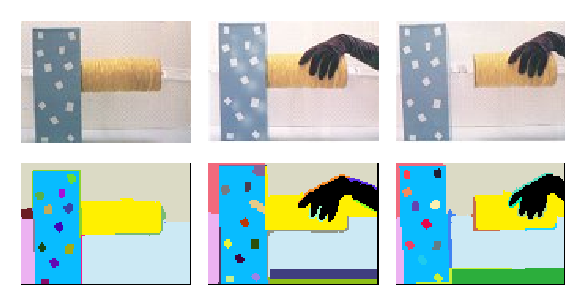
\includegraphics[width=0.5\columnwidth]{fig-pull}}

\caption{
Top: photos of one of Needhan's experiments; a yellow tube is 
pulled away from a blue box with white dots.
Bottom: segmentation of the photos.
}

\label{fig:move-apart}

\end{figure}

In this section we look at experiments that evaluate infant's
expectations about what should move together and what will move
independently; we will compare this to what is technically achievable.
For example, Figure~\ref{fig:move-apart} shows a scenario presented to
infants.



\begin{quote}

It is conceivable that young infants are not exposed to sufficient
contrastive evidence within the context of occlusion events. For
example, infants may seldom observe occlusion events in which: (a) the
objects seen to each side of an occluder either share, or do not
share, the same surface features; and (b) a judgment about the number
of objects present can only be made based on surface features. Without
such evidence, it would be difficult for infants to identify surface
features as important. Even once identified, infants may have few
opportunities to use, and to test, this new knowledge. If surface
features are indeed a less reliable source of information than form
features (e.g. see below), the opportunity to experiment with this new
knowledge might be necessary before infants would be disposed to use
it spontaneously. (Wilcox)

\end{quote}





\subsection{A technical evaluation of Gestalt principles}

How hard is spatiotemporal grouping?
Hard, in the general case.
Of a single, fixated object, while head is not moving much?  and
motion of head is available?

Still tough to do in real time, but the data is there in a form
we could process, given world enough and time.


Motion first -- then shape -- then color/pattern

What is there to learn about shape?  How to see it.

Needham 1999 result is not consistent with the direction of comp
vision research.  Algorithms would group two adjacent objects with
same color-and-pattern but different shapes long before grouping two
adjacent objects with same shape but different color-and-pattern.
Shape is inherently non-local, which color-and-pattern 
can at least to some extent be treated as a local feature.
Computationally, there 
has been little success in recovering shapes in cluttered static scenes.

Why could it make sense?  Lighting variation, color constancy is
really complicated -- maybe better to ignore until had a lot
of experience?

Appearance of surface is subject to a multiplicative effect
with its environment -- shadows, interreflections.

issue of 3D shape, 2D contours.

invariance versus selectivity, classic tradeoff.

If we start with motion, then what we have is motion silhouettes.
We can align the silhouette with the scene, and attempt to train
up methods for predicting the silhouette from the scene.
For a *particular* object at a particular time, it would seem 
best to use all the available correlated features, including 
surface features.  

Why would surface-info not be used in Needham1999 situation,
or be overridden by shape?

Suggest (1) train up generic boundary predictor, so
shape is perceivable, and (2) when shape is available,
segment based on it

Shape information is more important for actually doing things.

(could have more than silhouette from motion of course).


Shape in these particular experiments is maybe not that hard to
recover.

Maybe shape info is easier to use to link motion segmentation
events?  More trustworthy?  Cluster based on shape cues?

For my thesis, with a bunch of segmentations, clusturing by
some course shape measures gave around 88\% accuracy while
clustering by color histogram gave around 99\% accuracy.
But the robot was living in one corner of a lab, with 
relatively constant lighting.  In real life, the story may
be quite different.  Any evidence to suggest this?

Also, the development from grouping anything that moves
together, to then using gaps, is novel and interesting.
Get the cite.




\subsection{Possibilities}

``separately moving'' is not totally clear - consider e.g. a 
jacket, can move arms around a certain amount without body.

Bottom up or top down?  Bottom up and top down?  Interaction
with recognition?

Most commonly, but not always, segmentation is implemented
as a precursor to recognition.  Image comes in, gets
segmented, segments are then run through recognizer.

This is problematic, since segmentation without
recognition is relatively brittle -- it is uninformed.
For something like finding faces, it is more common
not to segment first -- but the common trick here
is to try all possible regions.

Good features, a progression.


\section{INTRO}


Johnson et al re segregation in the presence of partial occlusion.



\noindent General interests:

\begin{itemize}

\item Experiments that demonstrate ``development'' based on experience,
   particularly single or small numbers of episodes

\item Behaviors of the child/robot that have been demonstrated/argued
   to help generate good experience or otherwise help with development.

\end{itemize}


\subsection{Importance of motion?}

We are talking about the {\em development} of perception from an
immature form.  We assume that this development relies on acquiring
some information from the outside world (this isn't necessarily so).
How is this information acquired?  Sensory input is not 
uniformly difficult to interpret -- there are situations in
which it becomes simpler.  One particularly striking case is
the presence of motion.  Coherent group motion of part of the 
scene can be relatively easy to detect, and is a good cue for
the existence and extent of a corresponding object.  
So motion is one good place to start.
%
Moving objects are salient to infants and seem to play an
important role in perceptual learning (BACK THIS UP).
%
In robotics motion has frequently been used in all sorts of
ways.
%
Mention the technical status of motion detection versus
detection of other features (e.g. ``material'').
%
Of course this is by no means the end of the story, there 
are many other features... depth cues etc.

Egomotion is not very useful (relatively speaking).  Movemement of
others or caused by others is useful.  Motion caused by the robot
itself is particularly useful; this could be true of infants but is
moot given the limited motor control available initially.

\subsection{Preamble}

What is perception for?  One classic answer from robotics is that the
goal of perception is to recover, as faithfully as possible, the state
of the world.  That is, some model is made of the world, with some
number of free parameters, and the goal of perception is to find
values for those parameters to bring the model into as close an
alignment as possible with the world.

This view is my no means unquestioned; to achieve a particular
task, the most useful model to estimate may vary.  It may be
trivial, or the robot's behavior may be easier to produce or
describe in alternate ways that don't use the language of
model estimation.

In this paper, we will assume that the robot is engaged
in manipulation tasks (as opposed to, for example, navigation).

{\bf Behavioral view}: strategies that make it likely for the robot
to be looking somewhere useful (hand/eye coordination).
{\bf Model view}: ability to demonstrate flexible knowledge of presence of 
objects and some of their properties.


\subsection{Formalities}

Should provide the clearest possible definition of terms,
as a reference.  Human and robot uses of terms could deviate
from this definition if the deviation is also clearly described.

Object segregation, intermodal integration, object permanence.

Define a cell as the smallest sensing unit, for whichever sensors are
under consideration (e.g. pixels for images).  Assume there are a
fixed number of cells $c_1...c_{N}$.

There is also an unknown set of causes $s_1...s_{M}$, which for a
bounded period of consideration we will consider fixed.  Each cell
$c_i$ provides varying sensor readings $c_i(t)$.  We would like to
generate assignments $a_j(t)$ which, for each cause, lists all the
cells that can reasonably be attributed to that cause.  Then we choose
our causes to be maximally useful in describing the environment.

It is a little difficult to say exactly what judgement should be
made in complicated cases.  Might be better to give examples,
and underspecify.

Specification for object segregation:

$I(t) = [c_1.val(t) ... c_N.val(t)]$

Goal of segregation:
  Find a set $S_i$ = e.g. ${ c_2,c_4,c_5,c_6,... }$ that lists cells that
  belong together at a particular time.
  Find a set of such sets - Z.

Goal of intermodal integration:
  Bring together such sets across modal boundaries.

Goal of object permanence:
  Bring together such sets across time and disappearances.


***********

stuff to be integrated [from Lorenzo]:


The paper focuses on objects. Can we say something about the role of the
body? Achieving eye-hand coordination proved to be extremely useful on the
robots we have worked on. Learning to act is necessary to perform active
exploration of objects (poking/pushing/tapping/grasping). During action the
ability to identify the body helps the robot to focus the attention on the
area of the visual space where "things are happening" (i.e. on the hand upon
contact with the object).


***********

Big potential difference between infants and humans: the role
of manipulation in shaping early perception.  Infants can't
act that much to begin with.



\ifverbose

In this paper, we look for challenges that humans and robots share;
we look for problems in perception that can be addressed fruitfully
both in the simplified world of a robot and in experimental psychology.
%
In particular, we examine a perceptual skill~-- segregation or
segmentation~-- that has proven extremely challenging technically
in robotics, and particulary worthy of study in psychology.


Segregation/segmentation in robotics has the interesting property that
the difficulty of the problem varies greatly depending on the exact
scenario. ... non-homogeneous problems.


When we succeed in making a robot perform a task, then we've succeeded
in understanding it very deeply.

The fields of robotics and machine perception are devoted to
taking human abilities

work within this
robot-model of the world, developing algorithms 


A sad realization of the field of AI and robotics has been that
although our bodies and brains can easily and apparently effortlessly
interpret sensory experience and produce appropriate action,
it is a lot harder than it looks.



as scientists and engineers we have no idea how this is done.
In fact, we don't even know how it could possibly be done.


when we digitize our sensation and look
at the numbers, we're completely at a loss.  The problem isn't 
digitization~-- digital recordings of sounds and views, when reconstructed
and presented physically, are perfectly understandable.  The problem
is that


The field of robotics is obsessed with and expert in this model.
It turns out that even though...


Everything in robotics~-- the hardware, the algorithms, the
representations~-- is bound to this model.


%Robotics is fundamentally concerned with developing algorithms within
%this model which enable 

\fi
